\subsection{Mixed Reality und HoloLens}
\label{sec-2-1}

\subsubsection{Mixed Reality}
\label{sec-2-1-1}
\fbox{
	\parbox{\linewidth}{
		\textit{Ziel des Kapitels:}\\
		Begriffsklärung und Einordnung von AR,MR,VR in das Virtual Continuum. Wichtig für die Einordnung von MR in Education in Kap. \ref{sec-2-2}.\\[6px]
		\textit{Inhalte:}	
		\begin{itemize}
			\item Virtual Continuum erklären und AR, AV, VR einordnen
		\end{itemize}
		
		\textit{Wichtige Literatur:}	
		\begin{itemize}
			\item A taxonomy of mixed reality visual displays \cite{Milgram94}
			\item A survey of augmented reality \cite{Azuma97}
			\item Augmented Reality: Where we will all live \cite{Peddie17}
		\end{itemize}
}}

\begin{figure}[h!]
	\centering
	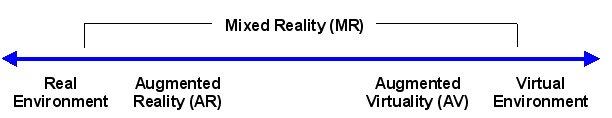
\includegraphics[width=0.9\textwidth]{images/virtual_continuum.png}
	\caption{Virtual Continuum eingeführt von Paul Milgram \cite{Milgram94}}
	\label{img:virtual_continuum}
\end{figure}

\begin{itemize}
	\item Kontinuierliches Spektrum zwischen real und virtuell
	\item MR ist Bereich zwischen völlig real und völlig virtuell, d.h. schließt AR und AV ein
	\item (optional) Einordnung von Beispielen HUD, Snapchat, Fragments, Oculus Rift
	\item Leistungssteigerung im Hardwarebereich und Fortschritte bei AI führt zur Verfügbarkeit von Devices von AR bis VR, daher sehr aktuelles Thema, viel Potential
\end{itemize}


\subsubsection{HoloLens}
\label{sec-2-1-2}
\fbox{
\parbox{\linewidth}{
	\textit{Ziel des Kapitels:}\\
	HoloLens und Mixed Reality Toolkit mit ihrer Technik und Interaktionsweise vorstellen.
}}\\

Die HoloLens ist ein von Microsoft entwickeltes \textit{Head-Mounted Display} (HMD), das seit 2016 auf dem Markt ist. Das Gerät ist in der Lage, virtuelle Darstellungen in der Umgebung des Trägers zu verankern und anzuzeigen. Abbildung \ref{img:hololens} zeigt die Brille in der Standardausführung. Die technischen Eigenschaften und genutzten Techniken des HMDs bringen verschiedene Implikationen und Einschränkungen für Anwendungen auf der HoloLens mit sich. Daher soll im Folgenden auf die technischen Aspekte näher eingegangen werden.\\

\begin{figure}[h!]
	\centering
	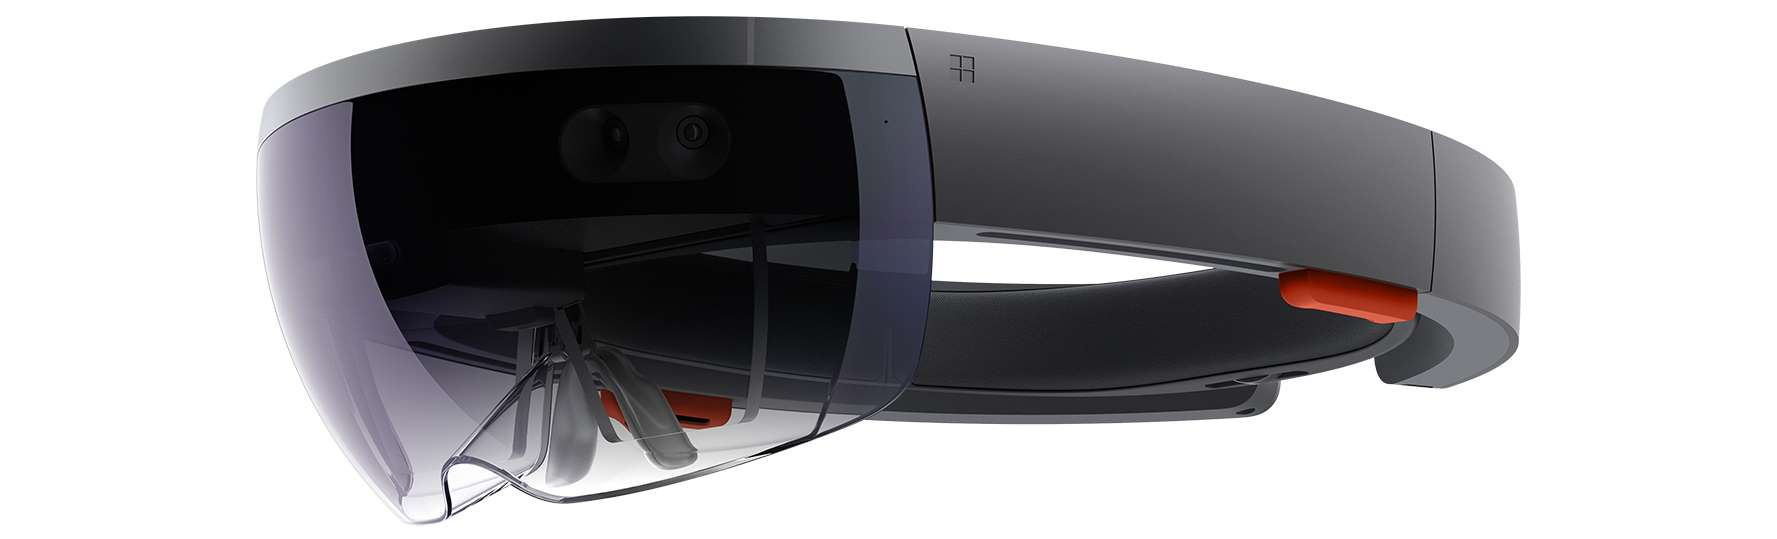
\includegraphics[width=0.9\textwidth]{images/hololens.jpg}
	\caption{Die HoloLens in der Developer Edition (Quelle: Microsoft)}
	%https://www.microsoft.com/de-de/hololens
	\label{img:hololens}
\end{figure}

Bei dem Device handelt es sich um einen eigenständigen Computer, auf dem eine spezielle Version von Windows 10 läuft. Die Brille arbeitet also völlig autonom und ist nicht auf externe Hardware wie z.B. zusätzliche Rechen- und Batterieeinheiten angewiesen.\\

\textbf{Die Hardware}\\
\begin{figure}[h!]
	\centering
	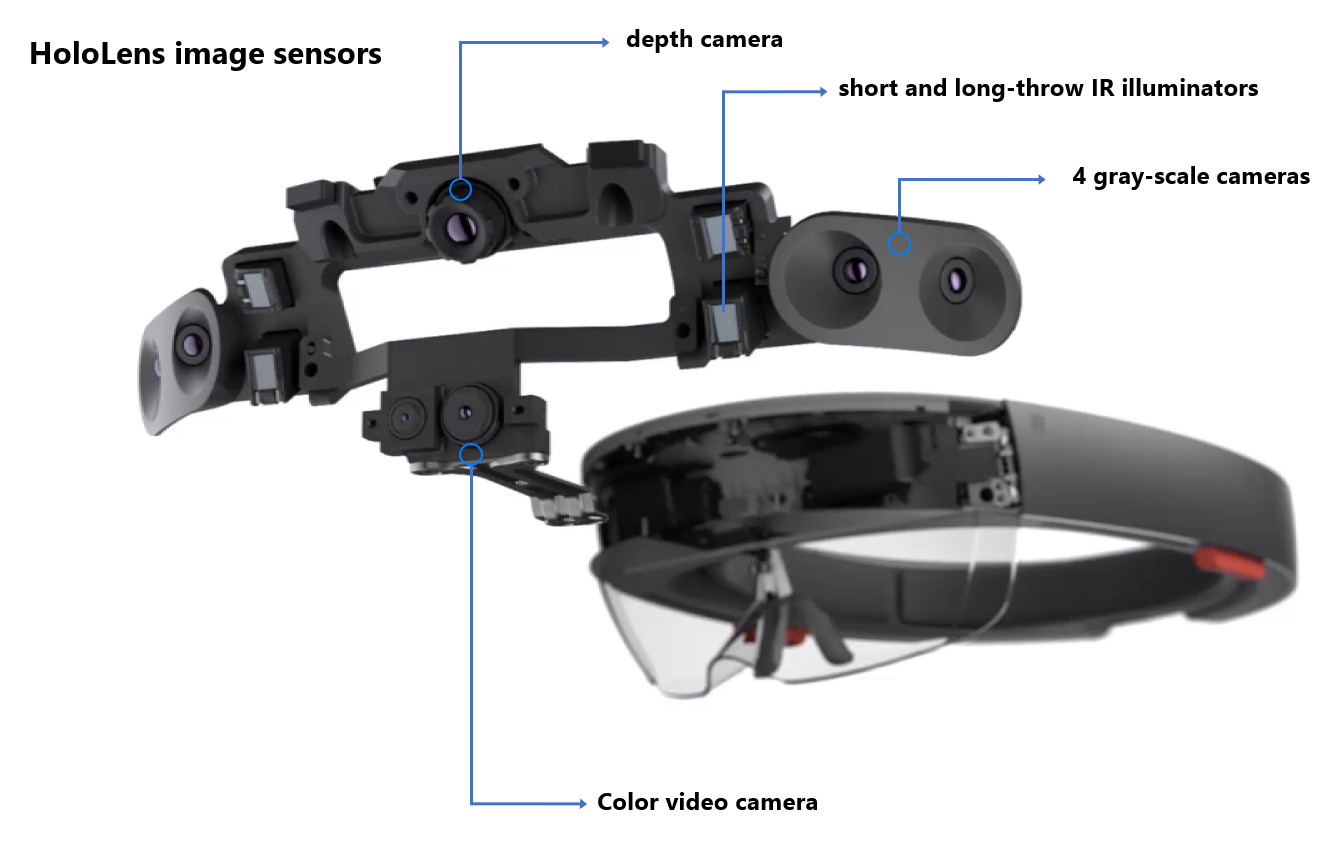
\includegraphics[width=0.9\textwidth]{images/hololens_tech.png}
	\caption{Die Sensorik der HoloLens (Quelle: Microsoft)}
	%https://docs.microsoft.com/en-us/windows/mixed-reality/hololens-hardware-details
	\label{img:hololens_tech}
\end{figure}

Einen Überblick über die verwendete Hardware gibt Tabelle \ref{tab:hololens_tech_details}.

\setlength\extrarowheight{2pt}
\begin{table}[htb]
	\centering
	\begin{tabular}{l|l}
		Kategorie & Eigenschaft\\
		\hline
		Anzeige & 720p (HD) in 16:9 Format pro Auge\\
		& 60 Hz Bildwiederholrate\\
		& Blickfeld ca. 32°\\
		Prozessor & Intel 32-Bit Prozessor @ 1.0 GHz\\
		Grafik & Microsoft Holographic Processing Unit (HPU)\\
		Arbeitsspeicher & 2 GB RAM\\
		& 1 GB HPU RAM\\
		Speicher & 64 GB Flash Speicher\\
		Kamera & 2 MP Foto / HD Video Front-Kamera\\
		Sensoren & Inertiale Messeinheit (Accelerometer, Gyroskop, Magnetometer) \\
		& Zwei Stereo Kameras\\
		& 120° x 120° Tiefenkamera\\
		& Vier Mikrofone\\
		& Ambient Light Sensor\\
		Power & 2-3h Akkulaufzeit \\
		Gewicht & 579 Gramm \\
		Konnektivität & WiFi, BLE, USB 2.0, 3.5 mm Audio Jack \\
		Steuerung & Gestensteuerung\\
		& Sprachsteuerung\\
		& HoloLens Klicker, Controller, Maus, Tastatur\\
	\end{tabular}\caption{\label{tab:hololens_tech_details} Spezifikation der HoloLens. Quelle: Microsoft}
\end{table}

\vspace{4px}
\textit{Das Display}\\
Kernstück des Gerätes ist das durchsichtige, stereoskopische Display, mit dem die virtuellen 3D-Objekte angezeigt werden. Durchsichtig bedeutet, dass das Display für Licht von außen durchlässig ist und der Nutzer somit wie durch eine Brille seine Umgebung sehen kann. Virtuelle Objekte werden zusätzlich dazu angezeigt, indem Licht über optische Wellenleiter (Optical Wave Guides) in das Display geleitet wird, welches das Licht dann auf die Augen reflektiert.\\

Anwendungen werden mit 60 Frames pro Sekunde dargestellt. Bei der Anzeige handelt es sich jedoch um ein \textit{Color Sequential Display}, bei dem die drei Farben Rot, Grün und Blau nacheinander dargestellt werden. Pro Bild werden folglich drei Einzelbilder (je eins pro Farbe) gezeigt, was eine Framerate von 240 Hz ergibt.\\

Es handelt sich dabei um ein stereoskopisches Display, bei dem pro Auge separat ein Bild dargestellt wird. So ermöglicht die HoloLens dem Träger das stereoskopische Wahrnehmen dreidimensionaler Objekte. Die beiden Bilder werden in einem festen Abstand von 22 mm zueinander dargestellt. Außerdem beträgt die Distanz, auf die sich die Augen einstellen müssen, damit Bilder als scharf wahrgenommen werden (Akkommodation), etwa zwei Meter und ist ebenfalls fest.\\

\vspace{4px}
\textit{Das Tracking}\\
Um die Hologramme im Raum verankern zu können, benötigt die HoloLens Informationen über ihre exakte Position und Orientierung im Raum. Beides erarbeitet das Gerät allein aus einem Zusammenspiel der verschiedenen internen Sensoren und ist nicht auf externe Markierungen angewiesen, es handelt sich um sogenanntes \textit{Inside-Out Tracking}. Das Vorgehen lässt sich dabei in zwei Bereiche unterteilen: Erfassen der unmittelbaren Umgebung sowie Orientierung anhand der Inertialmesssysteme.\\

Zum einen erstellt die HoloLens ein internes Modell der Oberflächenstruktur der Umgebung. Als Grundlage dazu dienen zum einen eine Tiefenkamera, die anhand der Time-of-Flight von ausgestrahltem Infrarotlicht die Entfernung zu nahegelegenen Oberflächen, die das Licht reflektieren, bestimmt. Zum anderen unterstützen die beiden Stereo-Kameras diese Informationen durch Triangulation von Objekten. Auf diese Weise erarbeitet die Brille ein 3D-Gitternetz, das nach und nach aktualisiert und vervollständigt wird, wenn sich der Träger im Raum bewegt. Anhand dieses sogenannten \textit{Spatial Mapping} wird ein Ankerpunkt für ein im Raum festes Koordinatensystem ausgewählt, dass der Brille als Referenzsystem dient.\\

Um die exakte Position und Ausrichtung der HoloLens nachzuverfolgen kommt außerdem die inertiale Messeinheit zum Einsatz. Die Beschleunigungs-, Rotations- und Magnetflusssensoren ermöglichen Schlussfolgerungen zu Änderungen in Position und Orientierung über eine Zeitdifferenz. Zusammen mit den Informationen aus den optischen Verfahren leitet die Brille so ihre genaue Position und Ausrichtung ab. Darüber hinaus speichert und unterscheidet das Gerät verschiedene Räume anhand der unterschiedlichen Struktur und den dort vorhandenen WLAN Signalen.\\


\textbf{Die Software und Interaktion}\\
Auf der HoloLens läuft eine spezielle Version von Windows 10: Windows 10 Holographic. Diese benötigt weniger Resourcen im Vergleich zu einem herkömmlichen PC und hat daher auch einen eingeschränkten Funktionsumfang. Anwendungen werden in Form von UWP Apps bereitgestellt. Hier unterstützt Microsoft die Entwicklung mit Unity und stellt entsprechende Toolkits zur Verfügung.\\

Die Steuerung durch den Nutzer erfolgt auf drei verschiedene Arten:
\begin{itemize}
	\item Handgesten
	\item Sprachbefehle
	\item Externe Eingabegeräte (Controller, Maus, Tastatur, etc.)
\end{itemize}

Erstere werden von der HoloLens automatisch erkannt und an die Anwendung in Form von Events weitergegeben, auf welche dann reagiert werden kann. Hier sind aktuell verschiedene Klick-Gesten zu nennen, durch die bekannte Mausfunktionen wie Klick, Click-and-Hold, Doppelklick und Drag-and-Drop abgebildet werden. Der Cursor orientiert sich dabei an der aktuellen Blickrichtung: Es wird automatisch das Objekt angeklickt, das als erstes von einer zentralen, vorwärts gerichteten Linie getroffen würde. Außerdem gibt es eine spezifische Handgeste zum aufrufen des Hauptmenüs.\\

Darüber hinaus nimmt die HoloLens englische Wörter als Sprachbefehle an, die sich auch kombinieren lassen. So kann eine Anwendung die Phrase "Hello World" als Keyword registrieren und dann darauf reagieren. Über Bluetooht lassen sich weitere Eingabegeräte anschließen: Den mit der HoloLens mitgelieferten Klicker, der die Klick-Geste ersetzen kann, aber auch eine Tastatur oder ein Controller lassen sich nutzen.\\

\textit{Das Mixed Reality Toolkit}\\
Das \textit{Mixed Reality Toolkit} (MRTK) ist ein quelloffenes Toolkit, das elementare Funktionen für die Entwicklung von Mixed Reality Anwendungen, insbesondere auch für die HoloLens, bereitstellt. Dazu gehört beispielsweise ein Objekt, das den zuvor genannten Cursor implementiert, aber auch Funktionen, die das Spatial Mapping auswerten. Für die Entwicklung mit Unity gibt es das Toolkit als Unitypackage, das unter anderem folgende Features bereitstellt:

\begin{itemize}
	\item Kameraobjekt mit den korrekten Einstellungen für die HoloLens
	\item Stabilisiertes Cursorobjekt mit Animationen für verschiedene Klicks
	\item Manager-Objekte, die Steuerung von Inputs und des Spatial Mappings erlauben
	\item Skripte für Standard Interaktionen wie Drag-and-Drop und Skalierung
	\item Für HoloLens angepasste Materialien und Shader
	\item Hilfsfunktionen wie z.B. eine FPS Anzeige oder mathematische Funktionen
\end{itemize}

Für die Entwicklung mit dem Toolkit und der HoloLens existiert ein umfassendes Repertoire aus Dokumentation, Beispielen, Guidelines, Einführungen und Hinweisen.\\


\textbf{Implikationen für Anwendungsdesign}\\
Genannte technische Details haben Auswirkung auf Nutzung und Design von Anwendungen
\begin{itemize}
	\item Stark spiegelnde oder transparente Materialien ungünstig für das Tracking
	\item Kein Schwarz darstellbar, Helligkeit im Raum relevant, Brille nur in Räumen zu verwenden
	\item Strenge Limitierung von Resourcen für Anwendung, da 60 FPS gehalten werden sollten, also keine komplexen Berechnungen möglich
	\item Abstand, Geschwindigkeit und Größe der Objekte wichtig, Blickwinkel
	\item GGf. Problem mit Sensorik der HoloLens (z.B. Magnetometer)
\end{itemize}
